\chapter{Literature Review}
This work has conducted a literature review and existing tool exploration to 
identify problem that provide motivation for research. This chapter also presents a running example. The running example is used throughout this thesis to help introducing and explaining concepts, such as presenting related work (e.g. incrementality, state/change-based model persistence and comparison), explaining this work's proposed approaches to address the slow loading of change-based models, and discussing how change-based model persistence can be exploited to optimise model differencing and conflict detection.

\section{Running Example}
\label{sec:running_example_1}
Let's say that there is a project to develop a simplified class diagram model of a Role Playing Game (RPG). Jane, as the technical leader, set up the initial model (Fig. \ref{fig:class_diagram_origin}). She then assigned this work to Bob and Alice. Both of them continued to work on the model and made some modification producing the models in Figures \ref{fig:class_diagram_left} and \ref{fig:class_diagram_right} respectively. Persisting these models in the standard XMI \cite{omg2018xmi} format produces three files as shown in Listings \ref{lst:xmimodel_origin}, \ref{lst:xmimodel_left}, and \ref{lst:xmimodel_right}.

\begin{figure}[ht]
  \begin{tabular}{l|c|r}
    \begin{subfigure}[t]{0.31\linewidth}
      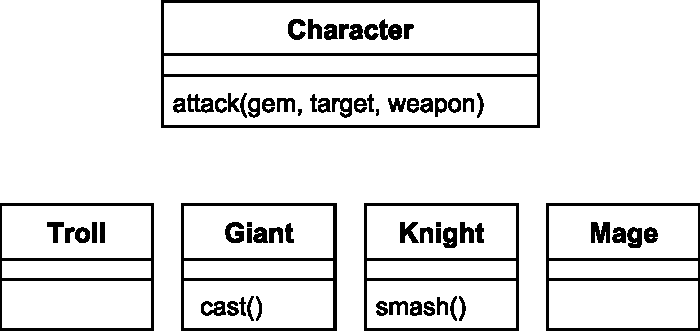
\includegraphics[width=\linewidth]{class_diagram_origin}
      \caption{original version (Jane's version)}
      \label{fig:class_diagram_origin}
    \end{subfigure}
    &
    \begin{subfigure}[t]{0.31\linewidth}
      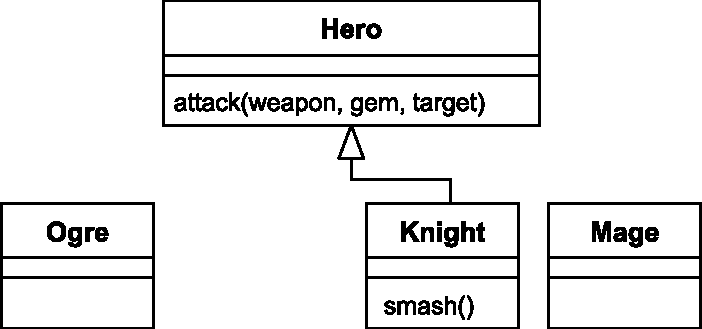
\includegraphics[width=\linewidth]{class_diagram_left}
      \caption{left version (Bob's version)}
      \label{fig:class_diagram_left}
    \end{subfigure}
    &
    \begin{subfigure}[t]{0.31\linewidth}
      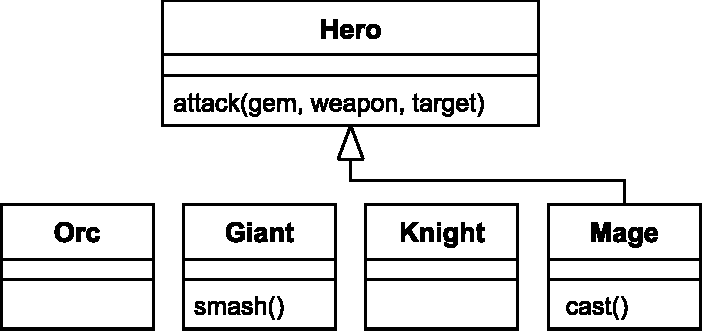
\includegraphics[width=\linewidth]{class_diagram_right}
      \caption{right version (Alice's version)}
      \label{fig:class_diagram_right}
    \end{subfigure}
  \end{tabular}
  \caption{Three class diagrams of a Role Playing Game.}
  \label{fig:class_diagram_rpg}
\end{figure}

\vspace{-20pt}
\begin{lstlisting}[style=xmi,caption={Simplified XMI file of the original version in Figure \ref{fig:class_diagram_origin}.},label=lst:xmimodel_origin]
<uml:Model>
  <packagedElement type=Class id="character" name="Character">
    <operation id="attack" name="attack">
      <parameter id="gem" name="gem"/>
      <parameter id="target" name="target"/>
      <parameter id="weapon" name="weapon"/>
    </operation>
  </packagedElement>
  <packagedElement type=Class id="troll" name="Troll"/>
  <packagedElement type=Class id="giant" name="Giant">
    <operation id="cast" name="cast"/>
  </packagedElement>
  <packagedElement type=Class id="knight" name="Knight">
    <operation id="smash" name="smash"/>
  </packagedElement>
  <packagedElement type=Class id="mage" name="Mage"/>
</uml:Model>
\end{lstlisting}

\vspace{-20pt}
\begin{lstlisting}[style=xmi,caption={Simplified XMI file of the left version in Figure \ref{fig:class_diagram_left}.},label=lst:xmimodel_left]
<uml:Model>
  <packagedElement type=Class id="character" name="Hero">
    <operation id="attack" name="attack">
      <parameter id="weapon" name="weapon"/>
      <parameter id="gem" name="gem"/>
      <parameter id="target" name="target"/>
    </operation>  
  </packagedElement>
  <packagedElement type=Class id="troll" name="Ogre"/>
  <packagedElement type=Class id="knight" name="Knight">
  <generalization id="leftGen" general="character"/>
    <operation id="smash" name="smash"/>
  </packagedElement>
  <packagedElement type=Class id="mage" name="Mage"/>
</uml:Model>
\end{lstlisting}

\vspace{-20pt}
\begin{lstlisting}[style=xmi,caption={Simplified XMI file of the right version of Figure \ref{fig:class_diagram_right}.},label=lst:xmimodel_right]
<uml:Model>
  <packagedElement type=Class id="character" name="Character">
    <operation id="attack" name="attack">
      <parameter id="gem" name="gem"/>
      <parameter id="weapon" name="weapon"/>
      <parameter id="target" name="target"/>
    </operation>
  </packagedElement>
  <packagedElement type=Class id="troll" name="Orc"/>
  <packagedElement type=Class id="giant" name="Giant">
    <operation id="smash" name="smash"/>
  </packagedElement>
  <packagedElement type=Class id="knight" name="Knight"/>
  <packagedElement type=Class id="mage" name="Mage">
    <generalization id="rightGen" general="character"/>
    <operation id="cast" name="cast"/>
  </packagedElement>
</uml:Model>
\end{lstlisting}

The company where Jane, Bob, and Alice work applies incremental model management in their development process. Applying incrementality allows them to manage their models automatically based on every change made to their models. For example, validating names of classes against a naming convention or to updating a class' documentation when the class is modified. Implementing this incrementality also comes with challenge and it is discussed in Section \ref{sec:the_key_challenge_of_incrementality}.



\section{The Key-Challenge of Incrementality}
\label{sec:the_key_challenge_of_incrementality}
To illustrate the key-challenge of incrementality, I use the example in Fig. \ref{fig:class_diagram_rpg}. Let's say that after every modification to the model in Fig. \ref{fig:class_diagram_origin}, the model needs to be:

\begin{itemize}
  \item Validated against a naming convention that the name of a class should start with an uppercase.
  \item Transformed into a number of documentation files through a model-to-text transformation. Each class should have a documentation file.
\end{itemize}

Models in Figures \ref{fig:class_diagram_origin} and \ref{fig:class_diagram_left} are two consecutive versions. When the validation constraint is evaluated against the first version of the model (Fig. \ref{fig:class_diagram_origin}), it verifies that all the classes' names starts with a uppercase, and the model-to-text transformation then produces four documentation files that correspond to the classes in the model. In the sequel, in Fig. \ref{fig:class_diagram_left}, the model is updated by Bob. He applies several changes, such as renaming class \textsf{Character} to \textsf{Hero} and class \textsf{Troll} to \textsf{Ogre} and deleting class \textsf{Giant}.

A non-incremental model validation engine would treat the model of 
Fig. \ref{fig:class_diagram_left} as if it was a new model and would evaluate 
the constraint above against every class in the model. 
An incremental model validation engine, on the other hand, would identify 
that the previously established satisfaction of the constraint for classes 
\textsf{Knight} and \textsf{Mage} cannot have been possibly compromised by the changes made, and would only re-evaluate the constraint for classes \textsf{Character} and \textsf{Troll} (class \textsf{Giant} is deleted so it is not evaluated). 

Similarly, a non-incremental model-to-text transformation would generate 
and overwrite all documentation files. On the contrary, an 
incremental model-to-text transformation, would identify that it only needs to delete the documentation file of class \textsf{Giant} and generate documentation files for classes \textsf{Character} and \textsf{Troll} -- but not the documentation files of classes \textsf{Knight} and \textsf{Mage}, as these cannot have been affected by the changes made to the model.

While the overhead of executing transformations and validation constraints 
on small models like the one in Fig. \ref{fig:class_diagram_origin} is negligible, non-incremental execution can become a significant bottleneck for large evolving models. As stressed in Selic's seminal work \cite{selic2003pragmatics}, with reference to model-to-text transformation, ``... \textsf{this is particularly true in the latter phases of the development cycle when programmers make many small changes as they fine-tune the system. To keep this overhead low, it is crucial for the code generators to have sophisticated change impact analysis capabilities that minimize the amount of code regeneration}''.

As demonstrated by the pioneering work of Egyed \cite{egyed2011automatically}, 
to achieve incremental re-execution of (deterministic) queries on 
structured models, an execution engine needs to:

\begin{enumerate}
  \item Record model element property accesses during the initial execution of the queries;
  \item Identify new and deleted elements and modified model element properties in the new version of the model;
  \item Combine the information collected in the steps above to identify the subset of (potentially) affected rules/queries/templates that need to be re-executed.
\end{enumerate}

To illustrate this, this example uses an OCL implementation of the domain-specific constraint in List. \ref{lst:constraint}.

\begin{lstlisting}[style=ocl,caption={OCL constraint requiring that a class should start with an uppercase.},label=lst:constraint]
context Class
inv UpperCase: self.name->subtring(1, 1) == self.name->subtring(1, 1)->toUpper()
\end{lstlisting}

\begin{table}[ht]
  \centering
  \caption{Property-access trace of the evaluation of the constraint in List. \ref{lst:constraint} on the model of Fig. \ref{fig:class_diagram_origin}.}
  \begin{tabular}{p{4cm} p{2.1cm} p{2cm} p{2.1cm}}
    \hline 
    \textbf{Constraint} & \textbf{Context} & \textbf{Accessed Element} & \textbf{Accessed Property} \\ 
    \hline 
    \textsf{Class.UpperCase}  & \textsf{character} & \textsf{character} & \textsf{name} \\ 
    \textsf{Class.UpperCase}  & \textsf{troll} & \textsf{troll} & \textsf{name} \\ 
    \textsf{Class.UpperCase}  & \textsf{giant} & \textsf{giant} & \textsf{name} \\ 
    \textsf{Class.UpperCase}  & \textsf{knight} & \textsf{knight} & \textsf{name} \\
    \textsf{Class.UpperCase}  & \textsf{mage} & \textsf{mage} & \textsf{name} \\
    \hline 
  \end{tabular} 
  \label{tab:property_access_trace}
\end{table}

During the initial evaluation of the constraint on the model of Fig. \ref{fig:class_diagram_origin}, an incremental OCL engine would compute the property access trace displayed in Table \ref{tab:property_access_trace} as a side-product. Now, when the model is updated (Fig. \ref{fig:class_diagram_left}), the execution engine can identify that:

\begin{itemize}
  \item There is an element deleted in the model (class \textsf{Giant}) for which the constraint is not necessary to be evaluated;
  \item The value of property \textsf{name} of classes \textsf{Character} and \textsf{Troll} have changed, and as such, the constrain needs to be re-evaluated on this elements.
\end{itemize}

Egyed has shown that the property-access recording approach is applicable to queries of arbitrary complexity, 
as long as they are deterministic. More recent work has shown that variants of this approach can be used to 
achieve incrementality in a wide range of model processing operations, including model-to-model 
transformation \cite{jouault2010towards}, model-to-text transformation \cite{DBLP:conf/ecmdafa/OgunyomiRK15}, 
model validation, and pattern matching \cite{DBLP:conf/ecmdafa/RathHV12}---as long as changes to models can be 
precisely identified (step 2 in the list above).

\section{Identifying Changes in Models}
\label{sec:identifying_changes_in models}
There are two approaches in the literature for identifying changes in models 
in order to enable incremental re-execution of model processing operations.

\textbf{Notifications}. In this approach, the incremental execution 
engine needs to hook into the notification facilities 
provided by the modelling tool through which the developer edits the model, 
so that the engine can directly receive notifications as soon as 
changes happen (e.g. class \textsf{giant} has been deleted, class \textsf{character} has been renamed to ``Hero''). 
This is an approach taken by the IncQuery incremental pattern matching 
framework \cite{DBLP:conf/ecmdafa/RathHV12} and the ReactiveATL incremental model-to-model 
transformation engine \cite{DBLP:conf/ecmdafa/OgunyomiRK15}. The main advantage of this 
approach is that precise and fine-grained change notifications are provided 
for free by the modelling tool (and thus do not need to be computed by the 
execution engine---which as discussed below can be expensive and inefficient). 
On the downside, this approach is a poor fit for collaborative development 
settings where modelling and automated model processing activities are 
performed by different members of the team.

\textbf{Model Differencing}. This approach eliminates the coupling between 
modelling tools and incremental execution engines. Instead of depending on 
live notifications, in this approach the developer in charge of automated model 
processing, needs to have access to a copy of the last version of the model that the model processing program (e.g. the model-to-text transformation) was 
executed upon, so that it can be compared against the current version of 
the model (e.g. using a model-differencing framework such as SiDiff or 
EMFCompare) and the delta can be computed on demand. The main advantage of 
this approach is that it works well in a collaborative development environment 
where typically developers have distinct roles and responsibilities. On the 
downside, model comparison and differencing are computationally expensive and 
memory-greedy (both versions of the model need to be loaded into memory before 
they can be compared), thus largely undermining the time and resource saving 
potentials of incremental re-execution. 

In summary, incremental model processing currently delivers significant 
performance benefits only in a single-developer environment where the modeller 
is also responsible for performing all the (incremental) model processing 
operations. As a result, in collaborative development environments, 
developers need to either forgo incremental model processing altogether 
or to work around this limitation by manually steering model processing 
programs to process only subsets of their models, which is cumbersome and 
error prone.

\section{A Novel Solution to Incrementality}
\label{sec:a_novel_solution_to_incrementality}
A novel solution to incrementality should be able to deliver the advantages of both notification and model differencing approaches while eliminate their drawbacks. To realize such solution, this work comes with an idea that models can be persisted in their complete history of changes, a.k.a. change-based model persistence, as opposed to state-based model persistence that persists models in their snapshots at a time. In change-based model persistence, information about changes that have been applied to models can be preserved, and the persistence can be shared across the members of a team, for example through Version Control Systems (e.g., SVN, Git).The proposed change-based model persistence is discussed later in Chapter \ref{ch:change_based_model_persitence}. 

Moreover, change-based model persistence also can be exploited to optimise model comparison to only compares versions of a model on parts that have only been changed since their last shared common version. In other words, not every element of the versions is compared which can lead to a faster model comparison. This solution is discussed later in Chapters \ref{ch:model_differencing} and \ref{ch:conflict_detection}. 

\section{Change vs. State-based Persistence}
\label{sec:change_based_vs_state_based_persistence}
The concept of change-based persistence is not new and has been used in persisting changes of software, object-oriented databases, hierarchical documents, and models 
\cite{DBLP:journals/entcs/RobbesL07,DBLP:conf/sde/LippeO92,DBLP:conf/caise/IgnatN05,koegel2010emfstore}. 

The nature of change-based persistence give us two advantages. First, it contains finer-granularity information (e.g. types of changes, the order of the changes, elements that were changed, previous values, etc.) of changes which can improve the accuracy of change detection \cite{DBLP:journals/entcs/RobbesL07,DBLP:conf/sde/LippeO92,DBLP:conf/caise/IgnatN05,mens2002state}. Second, it records changes ordered manner which means that changes made to a model can be identified sequentially without having to explore and compare all elements of compared versions of models \cite{DBLP:conf/edoc/KoegelHLHD10}. The advantages to detect changes more precisely and much faster can then have positive knock-on effects on supporting (1) developers compare and merge models in collaborative modelling environments \cite{DBLP:conf/sde/LippeO92,DBLP:conf/caise/IgnatN05,koegel2010emfstore}, and (2) incremental model management \cite{jouault2010towards,DBLP:conf/ecmdafa/OgunyomiRK15, DBLP:conf/ecmdafa/RathHV12}. Moreover, changed-based persistence contains abundant information which can be exploited for analytics \cite{DBLP:journals/entcs/RobbesL07}.


Nevertheless, change-based persistence also comes with downsides, such as ever-growing model files 
\cite{DBLP:journals/entcs/RobbesL07,DBLP:conf/edoc/KoegelHLHD10} and increased model loading time \cite{mens2002state}
which increase storage and computation costs. A model that is frequently modified will increase considerably in file size 
since every change is added to the file. The increased file size (proportional to the number of persisted changes) will, 
in turn, increase the loading time of the model since all changes have to be replayed to reconstruct the model's 
eventual state. 

These downsides have to be mitigated to enable the practical adoption of change-based persistence. 
One approach to reducing the file size of change-based models is by removing changes that do not affect the eventual 
state of the model. For the increased loading time, it can be mitigated by ignoring -- i.e. not replaying -- changes 
that are cancelled out by later changes or employing change-based and state-based persistence side-by-side so that the
benefits of state-based persistence on loading time can be obtained. 

Other downsides are change-based persistence requires 
integration with existing tools -- since it is still a non-standard approach -- for its adoption \cite{koegel2010emfstore}, 
and still has limited support for standard, text-based version controls for collaborative development \cite{koegel2010emfstore}. 
These downsides can be addressed by developing a change-based persistence plugin for a specific development environment 
(e.g. Eclipse) and persisting changes in text-based format to support text-based version controls (e.g. Git, SVN).

%3-layer metamodelling architectures such as EMF and MOF. 
\begin{table}[t!]
    \centering
    \caption{The advantages and downsides between change-based and state-based persistence.}
    \label{table:advantages_drawbacks}
    \begin{tabular}
        {|>{\centering\arraybackslash}p{1.1cm}|>{\centering\arraybackslash}p{1.1cm}|>{\centering\arraybackslash}p{5cm}|>{\centering\arraybackslash}p{5cm}|}
        \hline 
        \multicolumn{2}{|c|}{\textbf{Dimensions}}&\textbf{Change-based Approach}&\textbf{State-based Approach}\\
        \hline 
        \multicolumn{2}{|p{2.2cm}|}{\centering Advantages} &
        \begin{minipage}[t]{5cm}
            \raggedright
            \begin{itemize}[leftmargin=9pt]
                \setlength\itemsep{2pt}
                \item[-] Faster for detecting changes \cite{DBLP:conf/edoc/KoegelHLHD10}
                \item[-] More accurate, carry semantic information \cite{DBLP:journals/entcs/RobbesL07,DBLP:conf/sde/LippeO92,DBLP:conf/caise/IgnatN05,mens2002state}  
                \item[-] Faster and more accurate for comparison and merging \cite{DBLP:conf/sde/LippeO92,DBLP:conf/caise/IgnatN05,koegel2010emfstore}
                \item[-] Information carried is useful for analytics \cite{DBLP:journals/entcs/RobbesL07}
            \end{itemize}
        \end{minipage}
        & 
        \begin{minipage}[t]{5cm}
            \raggedright
            \begin{itemize}[leftmargin=9pt]
                \setlength\itemsep{2pt}
                \item[-] Faster for loading large models \cite{DBLP:conf/models/Espinazo-PaganCM11,daniel2016neoemf,eclipse2019cdo}
                \item[-] A default standard, no need integration with existing tools \cite{koegel2010emfstore}  
            \end{itemize}
        \end{minipage}
        \\
        \hline
        \multicolumn{2}{|p{2.2cm}|}{\centering Disadvantages} & \begin{minipage}[t]{5cm}
            \raggedright
            \begin{itemize}[leftmargin=9pt]
                \setlength\itemsep{2pt}
                \item[-] Increased record size \cite{DBLP:journals/entcs/RobbesL07,DBLP:conf/edoc/KoegelHLHD10}
                \item[-] Is not efficient for replaying (loading) for long records \cite{mens2002state}
                \item[-] Limited supports for standard, text-based version controls (e.g. GitHub) \cite{koegel2010emfstore} 
                \item[-] Not a standard, need integration with existing tools \cite{koegel2010emfstore} 
            \end{itemize}
        \end{minipage}
        & 
        \begin{minipage}[t]{5cm}
            \raggedright
            \begin{itemize}[leftmargin=9pt]
                \setlength\itemsep{2pt}
                \item[-] Slower for saving changes  \cite{mens2002state,daniel2016neoemf,DBLP:conf/models/Espinazo-PaganCM11}
                \item[-] Slower for comparison \cite{DBLP:conf/edoc/KoegelHLHD10}
                \item[-] Less accurate, does not carry semantic information \cite{mens2002state,DBLP:conf/edoc/KoegelHLHD10}  
            \end{itemize}
        \end{minipage}
        \\
        \hline
    \end{tabular} 
\end{table}

In contrast, state-based persistence has several advantages over change-based persistence. First, since it is the default standard of persisting models, most of the available modelling tools support this kind of persistence thus there is no need for integration with existing tools \cite{koegel2010emfstore}. Second, it is faster in loading models since there is no need to replay all changes as in change-based persistence. Also, applying lazy loading -- elements of models are not loaded upfront -- enable faster CRUD (create, read, update, delete) operations \cite{DBLP:conf/models/Espinazo-PaganCM11,daniel2016neoemf}. 

Compared to change-based persistence, state-based persistence has several downsides. First, it is slower than change-based persistence in saving changes \cite{mens2002state}. Even thought its backends already implemented lazy loading, it still needs to undergo certain indexing mechanism to persist changes \cite{daniel2016neoemf,DBLP:conf/models/Espinazo-PaganCM11,eclipse2019cdo}. Second, state-based persistence does not have any records of recent elements that have been changed in a model. Thus, every element has to be checked for differences which can be less efficient if the comparison is performed in change-based format \cite{DBLP:conf/edoc/KoegelHLHD10}. Third, since comparison in state-based format requires deriving differences through a diffing process -- not based on actual change records, it can be less accurate than comparison in change-based persistence which is provided with more information to detect changes accurately \cite{mens2002state,DBLP:conf/edoc/KoegelHLHD10}. The summary of 
the advantages and downsides between change-based and state-based persistence are presented in
Table \ref{table:advantages_drawbacks}.

\section{The State of Art of Model Persistence}
\label{sec:the_state_of_art_of_model_persistence}
By default, modelling tools that support the 3-layer metamodelling architectures of Eclipse Modelling Framework (EMF) \cite{steinberg2008emf} employ state-based persistence to persist models in Metadata Interchange (XMI) format. XMI is a standard issued by Object Management Group (OMG) for exchanging metadata information via Extensible Markup Language (XML) \cite{omg2018xmi}. 

There are several non-XMI approaches to state-based model persistence that use relational or NoSQL databases. For example, EMF Teneo \cite{eclipse2017teneo} persists EMF models in relational databases, while Morsa \cite{DBLP:conf/models/Espinazo-PaganCM11} persist models in documents with MongoDB backend \cite{mongodb}, and NeoEMF \cite{daniel2016neoemf} persists models in multi NoSQL backends (Graph, Map, Column). However, none of these approaches provides built-in support for versioning and models are eventually stored in binary files/folders which are known to be a poor fit for text-oriented version control systems like Git and SVN. Connected Data Objects (CDO) \cite{eclipse2019cdo}, which provides support for database-backed model persistence, also provides collaboration facilities, but CDO adoption necessitates the use of a separate version control system (e.g. a Git repository for code and a CDO repository for models), which introduces fragmentation and administration challenges \cite{barmpis2014evaluation}. Similar challenges arise in relation to other model-specific version control systems such as EMFStore \cite{koegel2010emfstore}.

\section{The State of Art of Model Comparison}
\label{sec:the_state_of_art_of_model_comparison}
The history of diffing can be tracked back to the presence of \textsf{diff} program on Unix or Unix-like platform \cite{hunt1976algorithm}. The program can perform diffing that is comparing text files ``in order to determine how or whether they differ'' \cite{diff}. Diffing basically is about finding the longest common subsequence between two or more sequences which commonly known as the Longest Common Subsequence (LCS) algorithms \cite{bergroth2000lcs}. This problem is equivalent to the Shortest Edit Script (SES) problem that is to find the smallest number of editing (add and delete) in order to make a sequence equal to another sequence \cite{DBLP:journals/algorithmica/Meyers86}. LCS or SES algorithms are commonly implemented by Version Control Systems, such as SVN \cite{svn-diff} and Git \cite{git-diff}, in their \textsf{diff} programs to identify differences between versions of files.   

Applying this diffing approach to some non-text artefacts, such as XML \cite{w3c-xml} and Ecore models \cite{steinberg2008emf}, is not straightforward since they have different characteristics to text files. For example, XML is a hierarchical document with a tree structure; one node can contains other nodes. The unique feature of XML is that its containment is  unordered whereas in text differencing order is a necessary feature. This has been addressed by Wang et al. \cite{wang2003xdiff} by exploiting key XML  structure characteristics. Diffing Ecore models is even more complex since the models support multiple characteristics of features, such as attribute/reference, literal/object values, single/multiple values, containment/non-containment, etc \cite{steinberg2008emf}. 

There are several existing tools for model differencing. Beyond EMF Compare \cite{emfcompare2018developer}, which this study used for comparative evaluation due to its maturity and ongoing development activity, tools such as SiDiff \cite{Treude2007SiDiff} and DSMDiff \cite{lin2009dsmdiff} also provide language-agnostic graph-based model comparison, with some room for configuration (e.g., assigning different weights to features of types in the language). Additional expressive power -- at the cost of increased complexity and configuration effort -- is offered by dedicated comparison languages such as the Epsilon Comparison Language, which can be used to compare both homogeneous and heterogeneous models \cite{kolovos2009ecl}. All of these tools works with state-based persistence to identify differences between models.

This work does not aware of any other work that targets comparison of change-based models persisted in text files. Only EMF Store \cite{koegel2010emfstore} identified addresses change-based model comparison but it persists models in its own dedicated backend system. Database-backed model persistence and version control solutions such as CDO \cite{eclipse2019cdo} and EMF Store provide diffing capabilities between different versions of the same model without requiring models to be fully loaded into memory, however they present integration challenges with mainstream software engineering tools (e.g., continuous integration systems, backup and restore facilities) which are typically file-based, and their performance can degrade as more models/users are added to a repository, since all models are effectively stored in a single database \cite{KolovosRMPGCLRV13}. 

\section{State-based Model Differencing}
\label{sec:state-based_model_differencing}
Referring to the example in Section \ref{sec:running_example_1}, at one time, Bob decides to compare his model to Alice's model because he is interested to analyse the differences between their models. Bob then uses a model differencing tool and perform state-based model differencing. 
In state-based model differencing, comparing models commonly consists of two steps: \emph{matching} and \emph{diffing}.
The matching process establishes matches between the elements of both models, to determine the elements in the left model that correspond to elements in the right model. Generally, the matching process iterates through all the elements of the models being compared and matches them by their identifiers or through a similarity mechanism  \cite{DBLP:conf/sfm/BroschKLSWW12,emfcompare2018developer}. The diffing process then identifies differences between the matched elements \cite{DBLP:conf/sfm/BroschKLSWW12,emfcompare2018developer}. 

In our example, the matching process in state-based comparison -- as performed by EMF Compare \cite{emfcompare2018developer} -- iterates through all the elements of both models and matches them using their identifiers. The matching process yields 10 matches: $m_1$ = (\textsf{character}, \textsf{character}), $m_2$ = (\textsf{attack}, \textsf{attack}), $m_3$ = (\textsf{gem}, \textsf{gem}), $m_4$ = (\textsf{weapon}, \textsf{weapon}), $m_5$ = (\textsf{target}, \textsf{target}), $m_6$ = (\textsf{troll}, \textsf{troll}), $m_7$ = (\textsf{knight}, \textsf{knight}), $m_8$ = (\textsf{smash}, \textsf{smash}), and $m_9$ = (\textsf{mage}, \textsf{mage}), and 3 unmatched elements, $um_1$ = (-, \textsf{giant}), $um_2$ = (-, \textsf{rightGen}), $m_3$ = (-, \textsf{cast}), and $um_4$ = (\textsf{leftGen}, -). 

The diffing process then iterates through all the matches and unmatched elements and uses an LCS algorithm to identify their differences. During iterating the matches, in the second match $m_2$, it identifies that, in order to make the left feature \textsf{parameters} equal to the right feature \textsf{parameters}, parameter \textsf{gem} has to be moved from index 1 to 0 (diff $ds_1$). It is important to note that the employed LCS algorithm does not detect the different position of parameter \textsf{weapon}; it only identifies the minimum number of differences which if all are resolved unidirectionally can make both models equal. Otherwise, the number becomes less optimal -- not minimum.

In the six match $m_6$, The diffing process identifies that the classes \textsf{troll} are different in their \textsf{name}. The left \textsf{troll}'s \textsf{name} is ``Ogre'' while the other \textsf{troll}'s \textsf{name} is ``Orc'' (diff $ds_2$). In the eight match $m_8$, the diffing process identifies that the containers of operation \textsf{smash} are different. Thus, element \textsf{smash} has to be move from \textsf{knight}'s \textsf{operations} to \textsf{giant}'s \textsf{operations} (diff $ds_3$). For the other matches, the diffing process does not identify any differences. 

From the unmatched elements ($um_1$, $um_2$, $um_3$, and $um_4$), the diffing process identifies that, in order to make the left model equal to the right model, class \textsf{giant} has to be added to the left model's resource at index 2 (diff $ds_4$), generalization \textsf{rightGen} has to be added to class \textsf{mage}' s \textsf{generalization} (diff $ds_5$), operation \textsf{cast} has to be added to class \textsf{mage}'s \textsf{operations} (diff $ds_6$), and  generalization \textsf{leftGen} has to be removed from class \textsf{knight}' s \textsf{generalization} (diff $ds_7$).

Differences are commonly expressed as a list of changes that must be applied to a target model so that it is made equal to a reference model. This work treats the left model as a reference model and the right model as the target model. This means that differences are expressed as changes applied to the right model so that it equals the left model. To express differences, this work uses the following terms: \textsf{LeftContainer}, \textsf{RightContainer}, \textsf{LeftFeature}, \textsf{RightFeature}, \textsf{LeftIndex}, \textsf{RightIndex}, \textsf{LeftValue}, \textsf{RightValue}, and \textsf{Kind}. The \textsf{*Container}, \textsf{*Feature}, and \textsf{*Value} are the target element, feature, and value involved in a difference (\textsf{*} symbol can be replaced with \textsf{Left} and \textsf{Right}). \textsf{*Index} is the index of a value in a feature. \textsf{Kind} is the type of difference. It can be one of these types: \textsf{CHANGE}, \textsf{ADD}, \textsf{DELETE}, and \textsf{MOVE}. \textsf{CHANGE} means a pair of single-valued features have different values. \textsf{ADD} indicates that a value does not exist in the right model, thus it requires the addition of the value. \textsf{DELETE} is the opposite of \textsf{ADD}. \textsf{MOVE} indicates that matched elements differ in terms of their containers, containing features, or indexes. A Container is an element that contains a value. A containing feature is a feature owned by a container in which a value is contained. An index is the position of a value in a containing feature.

Based on these definitions, this work can express the result of the diffing process as: $ds_{n}$ = [$LeftContainer_n$, $RightContainer_n$, $LeftFeature_n$, $RightFeature_n$, $LeftIndex_n$, $RightIndex_n$, $LeftValue_n$, $RightValue_n$, $Kind_n$]. Therefore:

$ds_{1}$ =  [\textsf{attack}, \textsf{attack}, \textsf{parameters}, \textsf{parameters}, 1, 0, \textsf{gem}, \textsf{gem}, \textsf{MOVE}]\\
$ds_{2}$ = [\textsf{troll}, \textsf{troll}, \textsf{name}, \textsf{name}, 0, 0, ``Ogre'', ``Orc'', \textsf{CHANGE}]\\
$ds_{3}$ = [\textsf{knight}, \textsf{giant}, \textsf{operations}, \textsf{operations}, 0, 0, \textsf{smash}, \textsf{smash}, \textsf{MOVE}]\\
$ds_{4}$ = [\textsf{resource}, \textsf{resource}, \textsf{null}, \textsf{null}, \textsf{null}, 2, \textsf{null}, \textsf{giant}, \textsf{ADD}]\\
$ds_{5}$ = [\textsf{knight}, \textsf{knight}, \textsf{generalization}, \textsf{generalization}, 0, 0, \textsf{leftGen}, \textsf{null}, \textsf{ADD}]\\
$ds_{6}$ = [\textsf{mage}, \textsf{mage}, \textsf{operations}, \textsf{operations}, \textsf{null}, 0, \textsf{null}, \textsf{cast}, \textsf{ADD}]\\
$ds_{7}$ = [\textsf{mage}, \textsf{mage}, \textsf{generalization}, \textsf{generalization}, 0, 0, \textsf{null}, \textsf{rightGen}, \textsf{DELETE}]

This work then can use this information to represent the differences visually as depicted in Fig. \ref{fig:xmi_comparison}. Applying these differences as changes to the right model will transform it into the left model.  

\begin{figure}
  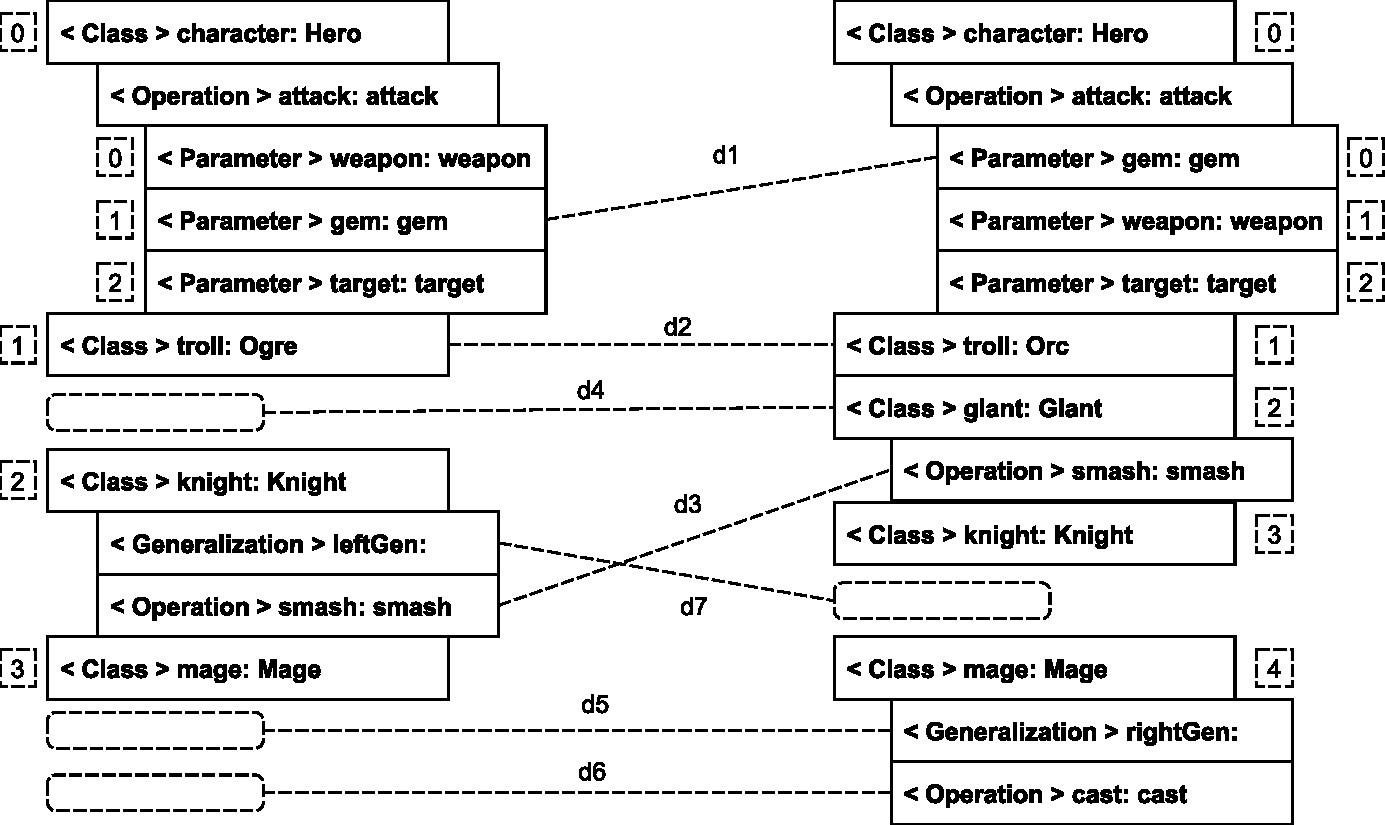
\includegraphics[width=\linewidth]{XmiComparison}
  \caption{A model comparison of the left and right models in Listings \ref{lst:xmimodel_left} and \ref{lst:xmimodel_right}.}
  \label{fig:xmi_comparison}
\end{figure}

\section{State-based Conflict Detection}
\label{sec:emfcompare_conflict_detection}
In state-based model comparison, the two sets of operations $O_{L}$ and $O_{R}$ are not readily available. They have to be derived trough model differencing. Both sets can be obtained by differencing $M_{L}$ to $M_{O}$ and $M_{R}$ to $M_{O}$ using an LCS algorithm as explained in Section \ref{sec:model_differencing}. These two differencing processes produce two sets of differences, $D_{OL}$ and $D_{OR}$, where $D_{OL}$ = $\{d_{ol1}$, $d_{ol2}$, ..., $d_{olg}\}$, $D_{OR}$ = $\{d_{or1}$, $d_{or2}$, ..., $d_{orh}\}$, and each difference $d$ is expressed as in (\ref{eq:diff_definition}). These differences can be treated as operations since if these differences are applied as operations to a target model, they transform it to become equivalent to a reference model. For example, applying a set of differences $D_{OL}$ to a model $M_{O}$ will transform it to model $M_{L}$. Therefore, it can be said that these differences are equivalent to operations. Thus, we can have two sets of operations, $O_{L}$ and $O_{R}$, which $O_{L} \equiv D_{OL}$ and $O_{R} \equiv D_{OR}$. These operations can then be used to detect conflicts using (\ref{eq:conflict_1.8}), (\ref{eq:conflict_1.9}), and (\ref{eq:conflict_1.10}).  

If EMF Compare is used to derive $O_{L}$ from Bob's and Jane's versions in Fig. \ref{fig:class_diagram_rpg} and present it in the format of change events, the following list are obtained. 
\begin{lstlisting}[firstnumber=1,style=eol,caption={The derived change events (operations) made by Bob to produce the right model in Fig. \ref{fig:class_diagram_left} (right version).},label=lst:cbp_left_state]
move target in attack.parameters from 1 to 2
set character.name from "Character" to "Hero"
set troll.name from "Troll" to "Ogre"
create leftGen type Generalization
set leftGen.general to character
set knight.generalization to leftGen
delete cast
delete giant
\end{lstlisting}

And following list is the derived change events for $O_{R}$ that are obtained from Bob's and Jane's versions in Fig. \ref{fig:class_diagram_rpg}. 
\begin{lstlisting}[firstnumber=1,style=eol,caption={The derived change events (operations) made by Alice to produce the right model in Fig. \ref{fig:class_diagram_right} (right version).},label=lst:cbp_right_state]
move gem in attack.parameters from 0 to 1
set character.name from "Character" to "Hero"
set troll.name from "Troll" to "Orc"
remove smash from knight.operations at 0
add smash to giant.operations at 0
create rightGen type Generalization
set rightGen.general to character
set mage.generalization to rightGen
remove cast from giant.operations at 1
add cast to mage.operations at 0
\end{lstlisting}

\textbf{Real Conflict}. In EMF Compare, a conflict occurs between two different operations, $o_{l}$ and $o_{r}$, if each is applied to a same element produce two different eventual states, where $!$ is the operator for expressing that two operations are in conflict. This conflict is classified \textsf{REAL} by EMF Compare.
\begin{equation} \label{eq:conflict_1.8}
e_{o} + o_{l} \not\equiv e_{o} + o_{r} \Rightarrow o_{l}\;!\;o_{r}
\end{equation} 
\textbf{Pseudo Conflict}. A conflict is classified as \textsf{PSEUDO} if the eventual states produced are equivalent. 
\begin{equation} \label{eq:conflict_1.9}
e_{o} + o_{l} \equiv e_{o} + o_{r} \Rightarrow o_{l}\;!_{p}\;o_{r}
\end{equation} 
\textbf{Non-applicability}. A conflict also occurs when applying operation $o_{l}$ to element $e_{o}$ makes $o_{r}$ inapplicable to element $e_{o}$. Therefore, operations $o_{l}$ and $o_{r}$ are in conflict. 
%For instance, Alice moved operation \textsf{smash} from class \textsf{Knight} to class \textsf{Giant} but this class was deleted by Bob. Deleting class \textsf{Giant} makes the move inapplicable. This conflict is classified \textsf{REAL} by EMF Compare.
\begin{equation} \label{eq:conflict_1.10}
(e_{o} + o_{r} \not\equiv e_{o}) \wedge (e_{o} + o_{l} + o_{r} \equiv e_{o} + o_{l}) \Rightarrow o_{l}\;!\;o_{r}
\end{equation}

\begin{table*}[]
  \centering
  \caption{Conflicting change events identified using EMF Compare based on the case in Fig. \ref{fig:class_diagram_rpg}.}
  \label{table:conflicts_emfc}
  % Please add the following required packages to your document preamble:
  % \usepackage[table,xcdraw]{xcolor}
  % If you use beamer only pass "xcolor=table" option, i.e. \documentclass[xcolor=table]{beamer}
  \begin{tabular}{|l|l|l|l|}
    \hline
    \multicolumn{1}{|c|}{{\color[HTML]{000000} \textbf{ID}}} & \multicolumn{1}{c|}{{\color[HTML]{000000} \textbf{Left Change Events (Bob)}}} & \multicolumn{1}{c|}{{\color[HTML]{000000} \textbf{Right Change Events (Alice)}}}                                      & \multicolumn{1}{c|}{{\color[HTML]{000000} \textbf{Type}}}           \\ \hline
    EC1                                                      & set character.name from "Character" to "Hero"                                 & set character.name from "Character" to "Hero"                                                                         & \begin{tabular}[c]{@{}l@{}}pseudo\\conflict\end{tabular} \\ \hline
    EC2                                                      & set troll.name from "Troll" to "Ogre"                                         & set troll.name from "Troll" to "Orc"                                                                                  & \begin{tabular}[c]{@{}l@{}}real conflict\end{tabular}        \\ \hline
    EC3                                                      & delete cast                                                                  & \begin{tabular}[c]{@{}l@{}}remove cast from giant.operations at 1\\ add cast to mage.operations at 0\end{tabular}     & \begin{tabular}[c]{@{}l@{}}non-\\ applicability\end{tabular}        \\ \hline
    EC4                                                      & delete giant                                                                   & \begin{tabular}[c]{@{}l@{}}remove smash from knight.operations at 0\\ add smash to giant.operations at 0\end{tabular} & \begin{tabular}[c]{@{}l@{}}non-\\ applicability\end{tabular}        \\ \hline
  \end{tabular}
\end{table*}

Using (\ref{eq:conflict_1.8}), (\ref{eq:conflict_1.9}), and (\ref{eq:conflict_1.10}) and information in Listings \ref{lst:cbp_right_state} and \ref{lst:cbp_left_state}, four conflicts can be identified -- presented in Table \ref{table:conflicts_emfc} along with their conflicting change events. Conflict \textsf{EC1} is a pseudo duality conflict since both modify the same class \textsf{character}'s feature \textsf{name} resulting the same end states, ``Hero'' or ``Hero''. Conflict \textsf{EC2} is a duality conflict. Applying changing \textsf{troll}'s \textsf{name} to ``Ogre'' and \textsf{troll}'s \textsf{name} to ``Orc'' produces two different states -- ``Ogre'' and ``Orc''. Conflicts \textsf{EC3} and \textsf{EC4} are non-applicability conflicts since if operation \textsf{cast} is deleted first then it cannot removed from class \textsf{giant}'s operations to be added to \textsf{mage}'s \textsf{operations}, and if class \textsf{giant} is deleted first then operation \textsf{smash} cannot be added to that class' operations.

Conflict detection in state-based comparison might not be accurate since the derived differences/operations might not reflect the real historical changes of a model.
For example, EMF Compare does not detect that Alice and Bob modified the same element -- parameter \textsf{target} -- as indicated by line 29 in List. \ref{lst:cbp_right} and line 35 in List. \ref{lst:cbp_left} . Using an LCS algorithm, the derived operations related to the feature \textsf{parameters} of element \textsf{attack}, which if presented as change events, are expressed as [\texttt{\small \textbf{move} target \textbf{in} attack.parameters \textbf{from} 1 \textbf{to} 2}] for Bob's version and [\texttt{\small \textbf{move} gem \textbf{in} attack. parameters \textbf{from} 1 \textbf{to} 2}] for Alice's version. Using (\ref{eq:conflict_1.3}), both operations are not in conflict since both operations modify two different elements, \textsf{target} and \textsf{gem}. The result is different if change-based approach is employed to detect conflicts using the change event records in Listings \ref{lst:cbp_right} and \ref{lst:cbp_left}. This is explained in Section \ref{sec:change_based_conflict_detection_emf_store}.

\section{Change-based Conflict Detection}
\label{sec:emfstore_l_conflict_detection}
\textbf{Non-commutability}. In EMF Store \cite{koegel2010emfstore} , operations $o_{l}$ and $o_{r}$ are in conflict if applying them in different order to a same element, in this case element $e_{o}$, produces two different eventual states.
\begin{equation} \label{eq:conflict_1.3}
e_{o} + o_{l} + o_{r} \not\equiv e_{o} + o_{l} + o_{r} \Rightarrow o_{l}\;!\;o_{r}
\end{equation} 
%For example, Alice changed the \textsf{name} of class \textsf{Troll} to ``Orc''while Bob renamed it to ``Ogre'' (Figure \ref{fig:class_diagram_rpg}). Applying Alice's change first to Bob's change results in the class' \textsf{name} equals to ``Ogre'', or ``Orc'' if the order is reversed. 
\textbf{Pseudo non-commutability}. However, after examining the implementation \footnote{\url{https://git.eclipse.org/c/emf-store}}, even though the eventual states are equivalent, both operations are still treated  in conflict. 
\begin{equation} \label{eq:conflict_1.5}
e_{o} + o_{l} + o_{r} \equiv e_{o} + o_{l} + o_{r} \Rightarrow o_{l}\;!_{p}\;o_{r}
\end{equation} 
\textbf{Non-applicability}. This non-applicability rule is the same with the non-applicability rule in the state-based conflict detection. The rule is presented again here. 
\begin{equation} \label{eq:conflict_1.6}
(e_{o} + o_{r} \not\equiv e_{o}) \wedge (e_{o} + o_{l} + o_{r} \equiv e_{o} + o_{l}) \Rightarrow o_{l}\;!\;o_{r}
\end{equation}
\textbf{Composite}. If operation $o_{l}$ is in conflict with operation $o_{r}$ where $o_{r}$ is a member of composite operation $co_{r}$ then operation $o_{l}$ is also in conflict with each operation $o_{n}$ in composite operation $co_{r}$.
%For example, deleting class \textsf{Giant} (List. \ref{lst:cbp_left} line 40) is not only in conflict with adding operation \textsf{smash} to class \textsf{Giant}'s operations (List. \ref{lst:cbp_right} line 31), but also with the removal of operation \textsf{smash} from class \text{Knight}'s operations (List. \ref{lst:cbp_right} line 31).
\begin{equation} \label{eq:conflict_1.7}
o_{l}\;!\;o_{r} \wedge o_{r} \in co_{r} \Rightarrow o_{l}\;!\; \forall o_{n} | o_{n} \in co_{r}
\end{equation}

\begin{table*}[]
  \centering
  \caption{Conflicting change events identified using EMF Store in Listings \ref{lst:cbp_right} and \ref{lst:cbp_left}.}
  \label{table:conflicts_emfs}
  \begin{tabular}{|l|l|l|l|}
    \hline
    \multicolumn{1}{|c|}{{\color[HTML]{000000} \textbf{ID}}} & \multicolumn{1}{c|}{{\color[HTML]{000000} \textbf{Left Change Events (Bob)}}}                                                                                                                                              & \multicolumn{1}{c|}{{\color[HTML]{000000} \textbf{Right Change Events (Alice)}}}                                                          & \multicolumn{1}{c|}{{\color[HTML]{000000} \textbf{Type}}}                                    \\ \hline
    \multirow{2}{*}{ES1} & set troll.generalization from null to leftGen                                                                                                                                                                              & \begin{tabular}[c]{@{}l@{}}unset troll.generalization from rightGen to null\\set mage.generalization from null to rightGen\end{tabular} & \multirow{2}{*}{\begin{tabular}[c]{@{}l@{}}non-\\ commutability, \\ composite\end{tabular}}                                                                                             \\ \cline{2-3}
    & \begin{tabular}[c]{@{}l@{}}unset troll.generalization from leftGen to null\\ set knight.generalization from null to leftGen\end{tabular}                                                                                   & set troll.generalization from null to rightGen                                                                                             &  \\ \hline
    ES2                                                      & set character.name from "Character" to"Hero"                                                                                                                                                                               & set character.name from "Character" to "Hero"                                                                                             & \begin{tabular}[c]{@{}l@{}}pseudo non-\\ commutability\end{tabular}                          \\ \hline
    ES3                                                      & move target in attack.parameters from 1 to 2                                                                                                                                                                               & move target in attack.parameters from 1 to 0                                                                                              & \begin{tabular}[c]{@{}l@{}}non-\\ applicability\end{tabular}                                 \\ \hline
    \multirow{2}{*}{ES4} & \multirow{2}{*}{\begin{tabular}[c]{@{}l@{}}unset cast.name from "cast" to null\\ remove cast from giant.operations at 0\\ delete cast type Operation\\ unset giant.name from "Giant" to null\\ delete giant\end{tabular}}                                                                                                                                                                                                                            & \begin{tabular}[c]{@{}l@{}}remove cast from giant.operations at 0\\ add cast to mage.operations at 0 \end{tabular}                         
    & \multirow{2}{*}{\begin{tabular}[c]{@{}l@{}}non-\\ applicability,\\ composite\end{tabular}} \\ \cline{3-3}
    &  & \begin{tabular}[c]{@{}l@{}}remove smash from knight.operations at 0\\ add smash to giant.operations at 1\\ \\ \\ \end{tabular}                     &   \\ \hline
    
    ES5                                                      & set troll.name from "Troll" to "Ogre"                                                                                                                                                                                      & set troll.name from "Troll" to "Orc"                                                                                                      & \begin{tabular}[c]{@{}l@{}}non-\\ commutability\end{tabular}                                 \\ \hline
  \end{tabular}
\end{table*}

In change-based conflict detection, all operations applied to a model are already available in change-based persistence, thus the operations do not need to be derived trough a diffing process. The availability of real historical changes can improve the accuracy of change detection since elements that have been changed can be identified accurately. In consequence, the undetected conflict in state-based conflict detection can be detected. For example, in Listing \ref{lst:cbp_right} line 29, parameter \textsf{target} has been moved from index 1 to 0, while in Listing \ref{lst:cbp_left} line 35, it was moved from index 1 to 2. Since both operations modified the same parameter \textsf{target}, using (\ref{eq:conflict_1.3}), both operations that are in conflict can be identified; parameter \textsf{target} are at different indexes if both operations are applied in different order, and \textsf{parameters}, the containing feature of \textsf{target}, is an ordered feature (Table \ref{table:conflicts_emfs} id ES1).  

The drawback of EMF Store is that it only performs comparison between operations to determine conflicts; it does no take into account the end states of models produced by the operations. In consequence, two operations are in conflict just by modifying a same element regardless of the end states that they produce to the element \cite{DBLP:conf/sfm/BroschKLSWW12}; there is no classification of conflicts to \textsf{REAL} or \textsf{PSEUDO} conflicts. For example, two operations represented by the two change events in Listing \ref{lst:cbp_right} at line 37 and Listing \ref{lst:cbp_right} at line 32, that change the same feature \textsf{name} to the same value ``Hero'', are treated in conflict (Table \ref{table:conflicts_emfs} id ES2). 

The inconsideration of eventual states also causes the assignments of generalizations \textsf{leftGen} and \textsf{rightGen} to class \textsf{troll}'s feature \textsf{generalization}, in Listings \ref{lst:cbp_right} at line 38 and \ref{lst:cbp_left} at line 33, to be in conflict with the \textsf{move} operations on the opposite sides (Table \ref{table:conflicts_emfs} id ES1). Setting feature \textsf{troll}'s \textsf{generalization} to element \textsf{leftGen} is in conflict with the \textsf{move} composite operation that moves \textsf{rightGen} from \textsf{troll}'s \textsf{generalization} to \textsf{mage}'s \textsf{generalization}. Using the non-commutability (\ref{eq:conflict_1.3}) and composite (\ref{eq:conflict_1.7}) rules, we can detect that executing these operations in different order causes \textsf{troll}'s \textsf{generalization} has two different eventual values; \textsf{troll}'s \textsf{generalization} is null if the \textsf{move} operation is executed first or \textsf{leftGen} if the \textsf{set} operation is executed first. We can use the same reasoning to explain the conflict between setting feature \textsf{troll}'s \textsf{generalization} to element \textsf{rightGen} and the \textsf{move} composite operation that moves \textsf{leftGen} from \textsf{troll}'s \textsf{generalization} to \textsf{knight}'s \textsf{generalization}.

In state-based conflict detection, the latter case (ES1) is not a conflict since the values of class \textsf{troll}'s feature \textsf{generalization} in the Jane's, Bob's, and Alice's versions are indentical -- all are null. Thus, there are no \textit{derived} operations that concurrently modify class \textsf{troll}'s feature \textsf{generalization}. Conflict ES4 is a non-applicability, composite conflict. Moving element \textsf{smash} from class \textsf{knight} to class \textsf{giant} and moving element \textsf{cast} from class \textsf{giant} to class \textsf{mage} require the deletion of class \textsf{giant} to be executed later in order to be applicable. Conflict ES5 is a non-commutability conflict. The \text{name} of class \textsf{troll} have an eventual value ``Ogre'' or ``Orc'' depending on the execution order of the conflicting operations.


